


\thispagestyle{empty}


%~
%\tikz[remember picture, overlay] \node  at (current page.center){\includegraphics[width=\paperwidth,height=\paperheight]{images/titlebg}};


~
\vskip 1.25in

\begin{flushright}
  \tikz[scale=0.6,yscale=.25]{\draw (0,0) rectangle (1,1);
  \draw (1.4,0) rectangle (3.4, 1) (3.8,0) rectangle (4.8,1) (4.8,0) rectangle (5.8,1); \draw (6.2,0) rectangle (8.2,1) (8.2,0) rectangle (9.2,1) (9.6,0) rectangle (10.6,1) (10.6,0) rectangle (12.6,1) (13,0) rectangle (14,1) (14,0) rectangle (15,1) (15,0) rectangle (16,1);
  }

  \vskip 2em

% \resizebox{\linewidth}{!}{\scshape Exploring Combinatorial Mathematics}
\resizebox{.4\linewidth}{!}{\scshape Exploring}

\vskip 1em
\resizebox{.65\linewidth}{!}{\scshape Combinatorial}

\vskip 1em
\resizebox{.55\linewidth}{!}{\scshape Mathematics}
\vskip 1em

% {\Huge\scshape Exploring}
% 
% \vskip 1em
% {\Huge\scshape Combinatorial}
% 
% \vskip 1em
% {\Huge \scshape Mathematics}
% \vskip 2em
\tikz[scale=0.6,yscale=.25]{\draw (0,0) rectangle (1,1);
\draw (1.4,0) rectangle (3.4, 1) (3.8,0) rectangle (4.8,1) (4.8,0) rectangle (5.8,1); \draw (6.2,0) rectangle (8.2,1) (8.2,0) rectangle (9.2,1) (9.6,0) rectangle (10.6,1) (10.6,0) rectangle (12.6,1) (13,0) rectangle (14,1) (14,0) rectangle (15,1) (15,0) rectangle (16,1);
}

\vskip 2em

% \resizebox{.25\linewidth}{!}{\scshape via Graph Theory}


%\tikz[scale=0.55]{\draw (0,0) rectangle (1,1);
%\draw (1.4,0) rectangle (3.4, 1) (3.8,0) rectangle (4.8,1) (4.8,0) rectangle (5.8,1); \draw (6.2,0) rectangle (8.2,1) (8.2,0) rectangle (9.2,1) (9.6,0) rectangle (10.6,1) (10.6,0) rectangle (12.6,1) (13,0) rectangle (14,1) (14,0) rectangle (15,1) (15,0) rectangle (16,1);
%}

\vskip 1.5in

\resizebox{.65\linewidth}{!}{\scshape Richard Grassl \& Oscar Levin}

\vskip .5in

\resizebox{.4\linewidth}{!}{\scshape 1st Edition, Fall 2019}

\end{flushright}


%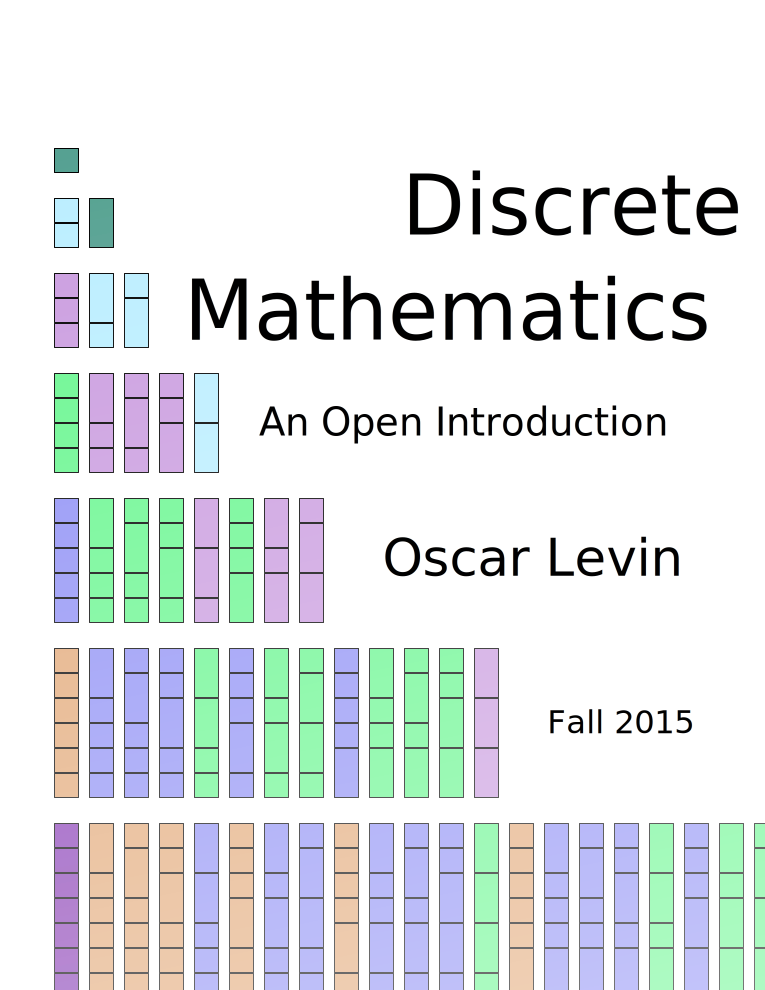
\includepdf[pages=-,pagecommand={\thispagestyle{empty}}]{frontmatter/cover2}
%
%

\clearpage






%\addtocontents{toc}{\protect\thispagestyle{plain}}
